\documentclass[UTF8,12pt,a4paper]{article}
%\documentclass[UTF8]{ctexart}
\usepackage{xltxtra,fontspec,xunicode}
\usepackage{graphicx} %允許載入圖片
\usepackage[colorlinks,linkcolor=black,urlcolor=blue]{hyperref}  %允許超連結
\usepackage[slantfont,boldfont]{xeCJK} % 允许斜体和粗体
\setCJKmainfont{STSongti-TC-Regular}   % 设置缺省中文字体
\setCJKmonofont{Hei}   % 设置等宽字体
\setmainfont{Optima}   % 英文衬线字体
\setmonofont{Monaco}   % 英文等宽字体
\setsansfont{Trebuchet MS} % 英文无衬线字体
% 導讀區
\title{《東方文化學刊》總目錄暨摘要}
\author{silentink}
\date{\today}
\begin{document}
\maketitle
\tableofcontents
\section{購買連結}
\subsection{\href{http://goods.ruten.com.tw/item/show?21607818417724url}{第一期}}
\subsection{\href{http://goods.ruten.com.tw/item/show?21607818426948}{第二期}  }
\subsection{\href{http://goods.ruten.com.tw/item/show?21537612540837}{第三期} } 
\subsection{\href{http://goods.ruten.com.tw/item/show?21607807273777}{第四期} } 
\subsection{\href{http://goods.ruten.com.tw/item/show?21633348062558}{第五期}  }

\paragraph{露天拍賣適用合併運費規則,一次買多本只須付一份運費。另外,也可以在奧丁丁網路開放市集購買全部:\url{https://www.owlting.com/market/items/1722}}

\paragraph{另,動畫《秘封活動記錄~月~第一話》DVD與前傳漫畫《月之追憶》的購買連結如下:url\{http://goods.ruten.com.tw/item/show?21607807078107}}
\section{簡介}
\paragraph{《東方文化學刊》是一本同人誌,以《東方Project》系列作及其同人文化為主題,創刊於2015年6月的台北,主編為「恆萃工坊」創辦人胡又天。這部同人誌的書名和內文格式都仿照正規學術期刊,為的是「給大家打氣」:證明遊戲、動漫和其他藝術形式一樣,當得起認真的研究與品評;透過發掘《東方Project》各作的歷史、民俗內涵,探討其中音樂、美術、遊戲設計等方面的學問,我們可以讓廣大同好更深入瞭解東方的世界,也為創作者提供借鑑,去作出更加精緻的作品。}
\paragraph{東方文化學刊》一、二期首發於2015年6月6日、在三重體育館舉辦的「博麗神社例大祭in 台灣」,第三期於9月出刊;2016年1月,前三期再版。第四期將首發於2016年2月21日、在台大綜合體育館舉辦的「Comic Horizon漫創地平線」活動中的「博麗神社例大祭 in台灣 1.5」區塊,攤位編號E13。}
\newpage

\section{第一期 3  同人于東方之野}
\begin{figure}[ht]
    \begin{center}
        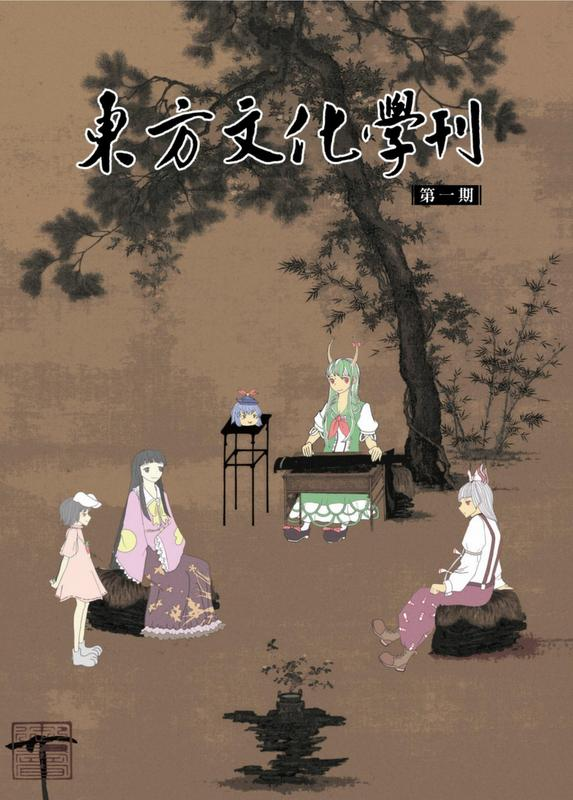
\includegraphics[width=10cm]{photo/1.jpg}
    \end{center}
\end{figure}
{題解:「同人于東方之野」典出《易經》〈同人〉卦辭:「同人于野,亨」;「野」(郊外)是相對於「國」(城裡人)的概念,在此即指相對於商業製作的同人創作。「東方之野」一方面表明本刊主題是東方Project,另一方面,也是對應《東方永夜抄》三面boss、掌握歷史的上白澤慧音的主題曲〈Plain Asia〉(或譯〈東方的平原〉)。}\\
% 換行
\paragraph{\bf 發刊詞:我們的心懷是博麗而永遠的}

{發刊詞宣示了在這個網路時代,仍選擇出版實體書的意義:一在向我們的社會宣示,又有一群認真對待電腦遊戲及動漫同人文化的成年人,要帶著多年積累的閱歷和知識,進來從事研究與評論了;二在為同好多提供一個寫作長文的誘因,以補網路隨筆之不足。然而,寫作不應是為了追求外在價值體系的認可,而應以藝術和我們的本心為依歸,故本文又提出「博麗精神」,希望大家能夠以無所拘繫的自在、自如來應對各色作品與這個世界。}
\end{document}





%%% Local Variables:
%%% mode: latex
%%% TeX-command-extra-options: "-shell-escape"
%%% TeX-master: t
%%% Tex-coding: utf-8
%%% TeX-engine: xetex
%%% End:



